%%
%% Automatically generated LaTeX file from Doconce source (http://code.google.com/p/doconce/)
%%
\documentclass{article}
\usepackage{hyperref,relsize,epsfig,makeidx}
\usepackage[latin1]{inputenc}
\usepackage{ptex2tex}
\usepackage{minted}  % requires latex -shell-escape (for Minted_* envirs)


\newcommand{\inlinecomment}[2]{  ({\bf #1}: \emph{#2})  }
%\newcommand{\inlinecomment}[2]{}  % turn off inline comments

\makeindex

\begin{document}

\newcommand{\x}{\pmb{x}}
\newcommand{\normalvec}{\pmb{n}}
\newcommand{\Ddt}[1]{\frac{D#1}{dt}}
\newcommand{\halfi}{1/2}
\newcommand{\half}{\frac{1}{2}}
\newcommand{\report}{test report}
\newcommand{\x}{\pmb{x}}
\newcommand{\normalvec}{\pmb{n}}
\newcommand{\Ddt}[1]{\frac{D#1}{dt}}




\begin{center}
{\LARGE\bf Doconce Description}
\end{center}



\begin{center}
{\bf Hans Petter Langtangen${}^{1, 2}$} \\ [0mm]
\end{center}

\begin{center}
{\small ${}^1$Simula Research Laboratory} \\ [-1.0mm]
\end{center}

\begin{center}
{\small ${}^2$University of Oslo} \\ [-1.0mm]
\end{center}

%\vspace{4mm}




\begin{center}
September 10, 2010
\end{center}


% lines beginning with # are comment lines


\section{What Is Doconce?}

\label{what:is:doconce}
\index{doconce!short explanation}

Doconce is two things:

\begin{enumerate}
 \item Doconce is a working strategy for documenting software in a single
    place and avoiding duplication of information. The slogan is:
    "Write once, include anywhere". This requires that what you write
    can be transformed to many different formats for a variety of
    documents (manuals, tutorials, books, doc strings, source code
    documentation, etc.).

 \item Doconce is a simple and minimally tagged markup language that can
    be used for the above purpose. That is, the Doconce format look
    like ordinary ASCII text (much like what you would use in an
    email), but the text can be transformed to numerous other formats,
    including HTML, Wiki, {\LaTeX}, PDF, reStructuredText (reST), Sphinx,
    Epytext, and also plain text (where non-obvious formatting/tags are
    removed for clear reading in, e.g., emails). From reStructuredText
    you can go to XML, HTML, {\LaTeX}, PDF, OpenOffice, and from the
    latter to RTF and MS Word.
\end{enumerate}

\noindent
The first point may be of interest even if you adopt a different
markup language than Doconce, e.g., reStructuredText or Sphinx.

So why not just use reStructuredText or Sphinx? Because Doconce

\begin{itemize}
  \item can convert to plain \emph{untagged} text, 
    more desirable for computer programs and email, 

  \item has less cluttered tagging of text,

  \item has better support for copying in computer code from other files,

  \item has stronger support for mathematical typesetting,

  \item works better as a complete or partial source for large {\LaTeX} 
    documents (reports and books).
\end{itemize}

\noindent
Anyway, after having written an initial document in Doconce, you may
convert to reStructuredText or Sphinx and work with that version for
the future.

Doconce was particularly written for the following sample applications:

\begin{itemize}
  \item Large books written in {\LaTeX}, but where many pieces (computer demos,
    projects, examples) can be written in Doconce to appear in other
    contexts in other formats, including plain HTML, Sphinx, or MS Word.

  \item Software documentation, primarily Python doc strings, which one wants
    to appear as plain untagged text for viewing in Pydoc, as reStructuredText
    for use with Sphinx, as wiki text when publishing the software at
    googlecode.com, and as {\LaTeX} integrated in, e.g., a master's thesis.

  \item Quick memos, which start as plain text in email, then some small
    amount of Doconce tagging is added, before the memos can appear as
    MS Word documents or in wikis.
\end{itemize}

\noindent
You can jump to Section~\ref{doconce:strategy} to see a recipe for
how to use Doconce, but first some more motivation for
the problem which Doconce tries to solve is presented.


\section{Motivation: Problems with Documenting Software}

\index{doconce!motivation}

\paragraph{Duplicated Information.}
It is common to write some software
documentation in the code (doc strings in Python, doxygen in C++,
javadoc in Java) while similar documentation is often also included in
a {\LaTeX} or HTML manual or tutorial. Although the various types of
documentation may start out to be the same, different physical files
must be used since very different tagging is required for different
output formats. Over time the duplicated information starts to
diverge. Severe problems with such unsynchronized documentation was
one motivation for developing the Doconce concept and tool.

\paragraph{Tagging Issues in Python Documentation.}
A problem with doc
strings in Python is that they benefit greatly from some tagging,
Epytext or reStructuredText, when transformed to HTML or PDF
manuals. However, such tagging looks annoying in Pydoc, which just
shows the pure doc string. For Pydoc we should have more minimal (or
no) tagging (students and newbies are in particular annoyed by any
unfamiliar tagging of ASCII text). On the contrary, manuals or
tutorials in HTML and {\LaTeX} need quite much tagging.

\paragraph{Solution.}
Accurate information is crucial and can only be
maintained in a \emph{single physical} place (file), which must be
converted (filtered) to suitable formats and included in various
documents (HTML/{\LaTeX} manuals/tutorials, Pydoc/Epydoc/HappyDoc
reference manuals).

\paragraph{A Common Format.}
There is no existing format and associated
conversion tools that allow a "singleton" documentation file to be
filtered to {\LaTeX}, HTML, XML, PDF, Epydoc, HappyDoc, Pydoc, \emph{and} plain
untagged text. As we are involved with mathematical software, the
{\LaTeX} manuals should have nicely typeset mathematics, while Pydoc,
Epydoc, and HappyDoc must show {\LaTeX} math in verbatim mode.
Unfortunately, Epytext is annoyed by even very simple {\LaTeX} math (also
in verbatim environments). To summarize, we need

\begin{enumerate}
 \item A minimally tagged markup language with full support for 
    for mathematics and verbatim computer code.

 \item Filters for producing highly tagged formats ({\LaTeX}, HTML, XML),
    medium tagged formats (reStructuredText, Epytext), and plain
    text with completely invivisble tagging. 

 \item Tools for inserting appropriately filtered versions of a "singleton"
    documentation file in other documents (manuals, tutorials, doc strings).
\end{enumerate}

\noindent
One answer to these points is the Doconce markup language, its associated
tools, and the \href{http://code.google.com/p/preprocess/}{C-style preprocessor tool}.
Then we can \emph{write once, include anywhere}!
And what we write is close to plain ASCII text.

But isn't reStructuredText exactly the format that fulfills the needs
above? Yes and no. Yes, because reStructuredText can be filtered to a
lot of the mentioned formats. No, because of the reasons listed
in Section~\ref{what:is:doconce}, but perhaps the strongest feature
of Doconce is that it integrates well with {\LaTeX}: Large {\LaTeX} documents (book)
can be made of many smaller Doconce units, typically describing examples
and computer codes, glued with mathematical pieces written entirely
in {\LaTeX} and with heavy cross-referencing of equations, as is usual
in mathematical texts. All the Doconce units can then be available
also as stand-alone examples in wikis or Sphinx pages and thereby used
in other occasions (including software documentation and teaching material).
This is a promising way of composing future books of units that can
be reused in many contexts and formats, currently being explored by
the Doconce maintainer.

A final warning may be necessary: The Doconce format is a minimalistic
formatting language. It is ideal when you start a new project when you
are uncertain about which format to choose. At some later stage, when
you need quite some sophisticated formatting and layout, you can
perform the final filtering of Doconce into something more appropriate
for future demands. The convenient thing is that the format decision
can be posponed (maybe forever - which is the common experience of the
Doconce developer).

\subsection{Dependencies}

Doconce depends on the Python package
\href{http://code.google.com/p/preprocess/}{preprocess}.  To make {\LaTeX}
documents (without going through the reStructuredText format) you also
need \href{http://code.google.com/p/ptex2tex}{ptex2tex} and some style files
that ptex2tex potentially makes use of.  Going from reStructuredText
to formats such as XML, OpenOffice, HTML, and {\LaTeX} requires
\href{http://docutils.sourceforge.net/}{docutils}.  Making Sphinx documents
requires of course \href{http://sphinx.pocoo.org}{sphinx}.

\subsection{The Doconce Software Documentation Strategy}

\label{doconce:strategy}

\begin{itemize}
   \item Write software documentation, both tutorials and manuals, in
     the Doconce format. Use many files - and never duplicate information!

   \item Use {\fontsize{10pt}{10pt}\verb!#include!} statements in source code (especially in doc
     strings) and in {\LaTeX} documents for including documentation
     files.  These documentation files must be filtered to an
     appropriate format by the program {\fontsize{10pt}{10pt}\verb!doconce2format!} before being
     included. In a Python context, this means plain text for computer
     source code (and Pydoc); Epytext for Epydoc API documentation, or
     the Sphinx dialect of reStructuredText for Sphinx API
     documentation; {\LaTeX} for {\LaTeX} manuals; and possibly
     reStructuredText for XML, Docbook, OpenOffice, RTF, Word.

   \item Run the preprocessor {\fontsize{10pt}{10pt}\verb!preprocess!} on the files to produce native
     files for pure computer code and for various other documents.
\end{itemize}

\noindent
Consider an example involving a Python module in a {\fontsize{10pt}{10pt}\verb!basename.p.py!} file.
The {\fontsize{10pt}{10pt}\verb!.p.py!} extension identifies this as a file that has to be
preprocessed) by the {\fontsize{10pt}{10pt}\verb!preprocess!} program. 
In a doc string in {\fontsize{10pt}{10pt}\verb!basename.p.py!} we do a preprocessor include
in a comment line, say
\begin{Verbatim}[fontsize=\fontsize{9pt}{9pt},tabsize=8,baselinestretch=0.85,
fontfamily=tt,xleftmargin=7mm]
#    #include "docstrings/doc1.dst.txt

\end{Verbatim}
\noindent
% 
% Note: we insert an error right above as the right quote is missing.
% Then preprocess skips the statement, otherwise it gives an error
% message about a missing file docstrings/doc1.dst.txt (which we don't
% have, it's just a sample file name). Also note that comment lines
% must not come before a code block for the rst/st/epytext formats to work.
% 
The file {\fontsize{10pt}{10pt}\verb!docstrings/doc1.dst.txt!} is a file filtered to a specific format
(typically plain text, reStructedText, or Epytext) from an original
"singleton" documentation file named {\fontsize{10pt}{10pt}\verb!docstrings/doc1.do.txt!}. The {\fontsize{10pt}{10pt}\verb!.dst.txt!}
is the extension of a file filtered ready for being included in a doc
string ({\fontsize{10pt}{10pt}\verb!d!} for doc, {\fontsize{10pt}{10pt}\verb!st!} for string).

For making an Epydoc manual, the {\fontsize{10pt}{10pt}\verb!docstrings/doc1.do.txt!} file is
filtered to {\fontsize{10pt}{10pt}\verb!docstrings/doc1.epytext!} and renamed to
{\fontsize{10pt}{10pt}\verb!docstrings/doc1.dst.txt!}.  Then we run the preprocessor on the
{\fontsize{10pt}{10pt}\verb!basename.p.py!} file and create a real Python file
{\fontsize{10pt}{10pt}\verb!basename.py!}. Finally, we run Epydoc on this file. Alternatively, and
nowadays preferably, we use Sphinx for API documentation and then the
Doconce {\fontsize{10pt}{10pt}\verb!docstrings/doc1.do.txt!} file is filtered to
{\fontsize{10pt}{10pt}\verb!docstrings/doc1.rst!} and renamed to {\fontsize{10pt}{10pt}\verb!docstrings/doc1.dst.txt!}. A
Sphinx directory must have been made with the right {\fontsize{10pt}{10pt}\verb!index.rst!} and
{\fontsize{10pt}{10pt}\verb!conf.py!} files. Going to this directory and typing {\fontsize{10pt}{10pt}\verb!make html!} makes
the HTML version of the Sphinx API documentation.

The next step is to produce the final pure Python source code. For
this purpose we filter {\fontsize{10pt}{10pt}\verb!docstrings/doc1.do.txt!} to plain text format
({\fontsize{10pt}{10pt}\verb!docstrings/doc1.txt!}) and rename to {\fontsize{10pt}{10pt}\verb!docstrings/doc1.dst.txt!}. The
preprocessor transforms the {\fontsize{10pt}{10pt}\verb!basename.p.py!} file to a standard Python
file {\fontsize{10pt}{10pt}\verb!basename.py!}. The doc strings are now in plain text and well
suited for Pydoc or reading by humans. All these steps are automated
by the {\fontsize{10pt}{10pt}\verb!insertdocstr.py!} script.  Here are the corresponding Unix
commands:

\vspace{4pt}
\begin{Verbatim}[numbers=none,frame=lines,label=\fbox{{\tiny Terminal}},fontsize=\fontsize{9pt}{9pt},
labelposition=topline,framesep=2.5mm,framerule=0.7pt]
# make Epydoc API manual of basename module:
cd docstrings
doconce2format epytext doc1.do.txt
mv doc1.epytext doc1.dst.txt
cd ..
preprocess basename.p.py > basename.py
epydoc basename

# make Sphinx API manual of basename module:
cd doc
doconce2format sphinx doc1.do.txt
mv doc1.rst doc1.dst.txt
cd ..
preprocess basename.p.py > basename.py
cd docstrings/sphinx-rootdir  # sphinx directory for API source
make clean
make html
cd ../..

# make ordinary Python module files with doc strings:
cd docstrings
doconce2format plain doc1.do.txt
mv doc1.txt doc1.dst.txt
cd ..
preprocess basename.p.py > basename.py

# can automate inserting doc strings in all .p.py files:
insertdocstr.py plain .
# (runs through all .do.txt files and filters them to plain format and
# renames to .dst.txt extension, then the script runs through all 
# .p.py files and runs the preprocessor, which includes the .dst.txt
# files)

\end{Verbatim}


% 
% some comment lines that do not affect any formatting
% these lines are simply removed
% 
% 
% 
% 
% 

\subsection{Demos}

\index{demos}

The current text is generated from a Doconce format stored in the
\vspace{4pt}
\begin{Verbatim}[numbers=none,frame=lines,label=\fbox{{\tiny Terminal}},fontsize=\fontsize{9pt}{9pt},
labelposition=topline,framesep=2.5mm,framerule=0.7pt]
docs/manual/manual.do.txt

\end{Verbatim}
file in the Doconce source code tree. We have made a 
\href{https://doconce.googlecode.com/hg/trunk/docs/demos/manual/index.html}{demo web page}
where you can compare the Doconce source with the output in many
different formats: HTML, {\LaTeX}, plain text, etc.

The file {\fontsize{10pt}{10pt}\verb!make.sh!} in the same directory as the {\fontsize{10pt}{10pt}\verb!manual.do.txt!} file
(the current text) shows how to run {\fontsize{10pt}{10pt}\verb!doconce2format!} on the
Doconce file to obtain documents in various formats.

Another demo is found in
\vspace{4pt}
\begin{Verbatim}[numbers=none,frame=lines,label=\fbox{{\tiny Terminal}},fontsize=\fontsize{9pt}{9pt},
labelposition=topline,framesep=2.5mm,framerule=0.7pt]
docs/tutorial/tutorial.do.txt

\end{Verbatim}
In the {\fontsize{10pt}{10pt}\verb!tutorial!} directory there is also a {\fontsize{10pt}{10pt}\verb!make.sh!} file producing a
lot of formats, with a corresponding
\href{https://doconce.googlecode.com/hg/trunk/docs/demos/tutorial/index.html}{web demo}
of the results.

% Example on including another Doconce file:


\section{From Doconce to Other Formats}

\label{doconce2formats}

Transformation of a Doconce document to various other
formats applies the script {\fontsize{10pt}{10pt}\verb!doconce2format!}:
\vspace{4pt}
\begin{Verbatim}[numbers=none,frame=lines,label=\fbox{{\tiny Terminal}},fontsize=\fontsize{9pt}{9pt},
labelposition=topline,framesep=2.5mm,framerule=0.7pt]
Unix/DOS> doconce2format format mydoc.do.txt

\end{Verbatim}
The {\fontsize{10pt}{10pt}\verb!preprocess!} program is always used to preprocess the file first,
and options to {\fontsize{10pt}{10pt}\verb!preprocess!} can be added after the filename. For example,
\vspace{4pt}
\begin{Verbatim}[numbers=none,frame=lines,label=\fbox{{\tiny Terminal}},fontsize=\fontsize{9pt}{9pt},
labelposition=topline,framesep=2.5mm,framerule=0.7pt]
Unix/DOS> doconce2format LaTeX mydoc.do.txt -Dextra_sections

\end{Verbatim}
The variable {\fontsize{10pt}{10pt}\verb!FORMAT!} is always defined as the current format when
running {\fontsize{10pt}{10pt}\verb!preprocess!}. That is, in the last example, {\fontsize{10pt}{10pt}\verb!FORMAT!} is
defined as {\fontsize{10pt}{10pt}\verb!LaTeX!}. Inside the Doconce document one can then perform
format specific actions through tests like {\fontsize{10pt}{10pt}\verb!#if FORMAT == "LaTeX"!}.

Inline comments in the text are removed from the output by
\vspace{4pt}
\begin{Verbatim}[numbers=none,frame=lines,label=\fbox{{\tiny Terminal}},fontsize=\fontsize{9pt}{9pt},
labelposition=topline,framesep=2.5mm,framerule=0.7pt]
Unix/DOS> doconce2format LaTeX mydoc.do.txt remove_inline_comments

\end{Verbatim}
One can also remove such comments from the original Doconce file
by running a helper script in the {\fontsize{10pt}{10pt}\verb!bin!} folder of the Doconce
source code:
\begin{Verbatim}[fontsize=\fontsize{9pt}{9pt},tabsize=8,baselinestretch=0.85,
fontfamily=tt,xleftmargin=7mm]
Unix/DOS> doconce_remove_inline_comments.py mydoc.do.txt

\end{Verbatim}
\noindent
This action is convenient when a Doconce document reaches its final form.

\subsection{HTML}

Making an HTML version of a Doconce file {\fontsize{10pt}{10pt}\verb!mydoc.do.txt!}
is performed by
\vspace{4pt}
\begin{Verbatim}[numbers=none,frame=lines,label=\fbox{{\tiny Terminal}},fontsize=\fontsize{9pt}{9pt},
labelposition=topline,framesep=2.5mm,framerule=0.7pt]
Unix/DOS> doconce2format HTML mydoc.do.txt

\end{Verbatim}
The resulting file {\fontsize{10pt}{10pt}\verb!mydoc.html!} can be loaded into any web browser for viewing.

\subsection{{\LaTeX}}

Making a {\LaTeX} file {\fontsize{10pt}{10pt}\verb!mydoc.tex!} from {\fontsize{10pt}{10pt}\verb!mydoc.do.txt!} is done in two steps:
% Note: putting code blocks inside a list is not successful in many
% formats - the text may be messed up. A better choice is a paragraph
% environment, as used here.

\paragraph{Step 1.}
Filter the doconce text to a pre-{\LaTeX} form {\fontsize{10pt}{10pt}\verb!mydoc.p.tex!} for
     {\fontsize{10pt}{10pt}\verb!ptex2tex!}:
\vspace{4pt}
\begin{Verbatim}[numbers=none,frame=lines,label=\fbox{{\tiny Terminal}},fontsize=\fontsize{9pt}{9pt},
labelposition=topline,framesep=2.5mm,framerule=0.7pt]
Unix/DOS> doconce2format LaTeX mydoc.do.txt

\end{Verbatim}
{\LaTeX}-specific commands ("newcommands") in math formulas and similar
can be placed in files {\fontsize{10pt}{10pt}\verb!newcommands.tex!}, {\fontsize{10pt}{10pt}\verb!newcommands_keep.tex!}, or
{\fontsize{10pt}{10pt}\verb!newcommands_replace.tex!} (see Section~\ref{newcommands}). 
If these files are present, they are included in the {\LaTeX} document 
so that your commands are defined.

\paragraph{Step 2.}
Run {\fontsize{10pt}{10pt}\verb!ptex2tex!} (if you have it) to make a standard {\LaTeX} file,
\vspace{4pt}
\begin{Verbatim}[numbers=none,frame=lines,label=\fbox{{\tiny Terminal}},fontsize=\fontsize{9pt}{9pt},
labelposition=topline,framesep=2.5mm,framerule=0.7pt]
Unix/DOS> ptex2tex mydoc

\end{Verbatim}
or just perform a plain copy,
\vspace{4pt}
\begin{Verbatim}[numbers=none,frame=lines,label=\fbox{{\tiny Terminal}},fontsize=\fontsize{9pt}{9pt},
labelposition=topline,framesep=2.5mm,framerule=0.7pt]
Unix/DOS> cp mydoc.p.tex mydoc.tex

\end{Verbatim}
Doconce generates a {\fontsize{10pt}{10pt}\verb!.p.tex!} file with some preprocessor macros.
For example, to enable font Helvetica instead of the standard
Computer Modern font,
\vspace{4pt}
\begin{Verbatim}[numbers=none,frame=lines,label=\fbox{{\tiny Terminal}},fontsize=\fontsize{9pt}{9pt},
labelposition=topline,framesep=2.5mm,framerule=0.7pt]
Unix/DOS> ptex2tex -DHELVETICA mydoc

\end{Verbatim}
The title, authors, and date are by default typeset in a non-standard
way to enable a nicer treatment of multiple authors having
institutions in common. The standard {\LaTeX} "maketitle" heading
is also available through
\vspace{4pt}
\begin{Verbatim}[numbers=none,frame=lines,label=\fbox{{\tiny Terminal}},fontsize=\fontsize{9pt}{9pt},
labelposition=topline,framesep=2.5mm,framerule=0.7pt]
Unix/DOS> ptex2tex -DTRAD_LATEX_HEADING mydoc

\end{Verbatim}

The {\fontsize{10pt}{10pt}\verb!ptex2tex!} tool makes it possible to easily switch between many
different fancy formattings of computer or verbatim code in {\LaTeX}
documents. After any {\fontsize{10pt}{10pt}\verb!!bc sys!} command in the Doconce source you can
insert verbatim block styles as defined in your {\fontsize{10pt}{10pt}\verb!.ptex2tex.cfg!}
file, e.g., {\fontsize{10pt}{10pt}\verb!!bc sys cod!} for a code snippet, where {\fontsize{10pt}{10pt}\verb!cod!} is set to
a certain environment in {\fontsize{10pt}{10pt}\verb!.ptex2tex.cfg!} (e.g., {\fontsize{10pt}{10pt}\verb!CodeIntended!}).
There are over 30 styles to choose from.

\paragraph{Step 3.}
Compile {\fontsize{10pt}{10pt}\verb!mydoc.tex!}
and create the PDF file:
\vspace{4pt}
\begin{Verbatim}[numbers=none,frame=lines,label=\fbox{{\tiny Terminal}},fontsize=\fontsize{9pt}{9pt},
labelposition=topline,framesep=2.5mm,framerule=0.7pt]
Unix/DOS> latex mydoc
Unix/DOS> latex mydoc
Unix/DOS> makeindex mydoc   # if index
Unix/DOS> bibitem mydoc     # if bibliography
Unix/DOS> latex mydoc
Unix/DOS> dvipdf mydoc

\end{Verbatim}
If one wishes to use the {\fontsize{10pt}{10pt}\verb!Minted_Python!}, {\fontsize{10pt}{10pt}\verb!Minted_Cpp!}, etc., environments
in {\fontsize{10pt}{10pt}\verb!ptex2tex!} for typesetting code, the {\fontsize{10pt}{10pt}\verb!minted!} {\LaTeX} package is needed.
This package is included by running {\fontsize{10pt}{10pt}\verb!doconce2format!} with the
{\fontsize{10pt}{10pt}\verb!-DMINTED!} option:
\vspace{4pt}
\begin{Verbatim}[numbers=none,frame=lines,label=\fbox{{\tiny Terminal}},fontsize=\fontsize{9pt}{9pt},
labelposition=topline,framesep=2.5mm,framerule=0.7pt]
Unix/DOS> ptex2tex -DMINTED mydoc

\end{Verbatim}
In this case, {\fontsize{10pt}{10pt}\verb!latex!} must be run with the
{\fontsize{10pt}{10pt}\verb!-shell-escape!} option:
\vspace{4pt}
\begin{Verbatim}[numbers=none,frame=lines,label=\fbox{{\tiny Terminal}},fontsize=\fontsize{9pt}{9pt},
labelposition=topline,framesep=2.5mm,framerule=0.7pt]
Unix/DOS> latex -shell-escape mydoc
Unix/DOS> latex -shell-escape mydoc
Unix/DOS> makeindex mydoc   # if index
Unix/DOS> bibitem mydoc     # if bibliography
Unix/DOS> latex -shell-escape mydoc
Unix/DOS> dvipdf mydoc

\end{Verbatim}
The {\fontsize{10pt}{10pt}\verb!-shell-escape!} option is required because the {\fontsize{10pt}{10pt}\verb!minted.sty!} style
file runs the {\fontsize{10pt}{10pt}\verb!pygments!} program to format code, and this program
cannot be run from {\fontsize{10pt}{10pt}\verb!latex!} without the {\fontsize{10pt}{10pt}\verb!-shell-escape!} option.

\subsection{Plain ASCII Text}

We can go from Doconce "back to" plain untagged text suitable for viewing
in terminal windows, inclusion in email text, or for insertion in
computer source code:
\vspace{4pt}
\begin{Verbatim}[numbers=none,frame=lines,label=\fbox{{\tiny Terminal}},fontsize=\fontsize{9pt}{9pt},
labelposition=topline,framesep=2.5mm,framerule=0.7pt]
Unix/DOS> doconce2format plain mydoc.do.txt  # results in mydoc.txt

\end{Verbatim}

\subsection{reStructuredText}

Going from Doconce to reStructuredText gives a lot of possibilities to
go to other formats. First we filter the Doconce text to a
reStructuredText file {\fontsize{10pt}{10pt}\verb!mydoc.rst!}:
\vspace{4pt}
\begin{Verbatim}[numbers=none,frame=lines,label=\fbox{{\tiny Terminal}},fontsize=\fontsize{9pt}{9pt},
labelposition=topline,framesep=2.5mm,framerule=0.7pt]
Unix/DOS> doconce2format rst mydoc.do.txt

\end{Verbatim}
We may now produce various other formats:
\vspace{4pt}
\begin{Verbatim}[numbers=none,frame=lines,label=\fbox{{\tiny Terminal}},fontsize=\fontsize{9pt}{9pt},
labelposition=topline,framesep=2.5mm,framerule=0.7pt]
Unix/DOS> rst2html.py  mydoc.rst > mydoc.html # HTML
Unix/DOS> rst2latex.py mydoc.rst > mydoc.tex  # LaTeX
Unix/DOS> rst2xml.py   mydoc.rst > mydoc.xml  # XML
Unix/DOS> rst2odt.py   mydoc.rst > mydoc.odt  # OpenOffice

\end{Verbatim}
The OpenOffice file {\fontsize{10pt}{10pt}\verb!mydoc.odt!} can be loaded into OpenOffice and
saved in, among other things, the RTF format or the Microsoft Word format.
That is, one can easily go from Doconce to Microsoft Word.

\subsection{Sphinx}

Sphinx documents can be created from a Doconce source in a few steps.

\paragraph{Step 1.}
Translate Doconce into the Sphinx dialect of
the reStructuredText format:
\vspace{4pt}
\begin{Verbatim}[numbers=none,frame=lines,label=\fbox{{\tiny Terminal}},fontsize=\fontsize{9pt}{9pt},
labelposition=topline,framesep=2.5mm,framerule=0.7pt]
Unix/DOS> doconce2format sphinx mydoc.do.txt

\end{Verbatim}

\paragraph{Step 2.}
Create a Sphinx root directory with a {\fontsize{10pt}{10pt}\verb!conf.py!} file, 
either manually or by using the interactive {\fontsize{10pt}{10pt}\verb!sphinx-quickstart!}
program. Here is a scripted version of the steps with the latter:
\vspace{4pt}
\begin{Verbatim}[numbers=none,frame=lines,label=\fbox{{\tiny Terminal}},fontsize=\fontsize{9pt}{9pt},
labelposition=topline,framesep=2.5mm,framerule=0.7pt]
mkdir sphinx-rootdir
sphinx-quickstart <<EOF
sphinx-rootdir
n
_
Name of My Sphinx Document
Author
version
version
.rst
index
n
y
n
n
n
n
y
n
n
y
y
y
EOF

\end{Verbatim}

\paragraph{Step 3.}
Move the {\fontsize{10pt}{10pt}\verb!tutorial.rst!} file to the Sphinx root directory:
\vspace{4pt}
\begin{Verbatim}[numbers=none,frame=lines,label=\fbox{{\tiny Terminal}},fontsize=\fontsize{9pt}{9pt},
labelposition=topline,framesep=2.5mm,framerule=0.7pt]
Unix/DOS> mv mydoc.rst sphinx-rootdir

\end{Verbatim}
If you have figures in your document, the relative paths to those will
be invalid when you work with {\fontsize{10pt}{10pt}\verb!mydoc.rst!} in the {\fontsize{10pt}{10pt}\verb!sphinx-rootdir!}
directory. Either edit {\fontsize{10pt}{10pt}\verb!mydoc.rst!} so that figure file paths are correct,
or simply copy your figure directory to {\fontsize{10pt}{10pt}\verb!sphinx-rootdir!} (if all figures
are located in a subdirectory).

\paragraph{Step 4.}
Edit the generated {\fontsize{10pt}{10pt}\verb!index.rst!} file so that {\fontsize{10pt}{10pt}\verb!mydoc.rst!}
is included, i.e., add {\fontsize{10pt}{10pt}\verb!mydoc!} to the {\fontsize{10pt}{10pt}\verb!toctree!} section so that it becomes
\begin{Verbatim}[fontsize=\fontsize{9pt}{9pt},tabsize=8,baselinestretch=0.85,
fontfamily=tt,xleftmargin=7mm]
.. toctree::
   :maxdepth: 2

   mydoc

\end{Verbatim}
\noindent
(The spaces before {\fontsize{10pt}{10pt}\verb!mydoc!} are important!)

\paragraph{Step 5.}
Generate, for instance, an HTML version of the Sphinx source:
\vspace{4pt}
\begin{Verbatim}[numbers=none,frame=lines,label=\fbox{{\tiny Terminal}},fontsize=\fontsize{9pt}{9pt},
labelposition=topline,framesep=2.5mm,framerule=0.7pt]
make clean   # remove old versions
make html

\end{Verbatim}
Many other formats are also possible.

\paragraph{Step 6.}
View the result:
\vspace{4pt}
\begin{Verbatim}[numbers=none,frame=lines,label=\fbox{{\tiny Terminal}},fontsize=\fontsize{9pt}{9pt},
labelposition=topline,framesep=2.5mm,framerule=0.7pt]
Unix/DOS> firefox _build/html/index.html

\end{Verbatim}

Note that verbatim code blocks can be typeset in a variety of ways
depending the argument that follows {\fontsize{10pt}{10pt}\verb!!bc!}: {\fontsize{10pt}{10pt}\verb!cod!} gives Python
({\fontsize{10pt}{10pt}\verb!code-block:: python!} in Sphinx syntax) and {\fontsize{10pt}{10pt}\verb!cppcod!} gives C++, but
all such arguments can be customized both for Sphinx and {\LaTeX} output.

% Desired extension: sphinx can utilize a "pycod" or "c++cod"
% instruction as currently done in latex for ptex2tex and write
% out the right code block name accordingly.

\subsection{Google Code Wiki}

There are several different wiki dialects, but Doconce only support the
one used by \href{http://code.google.com/p/support/wiki/WikiSyntax}{Google Code}.
The transformation to this format, called {\fontsize{10pt}{10pt}\verb!gwiki!} to explicitly mark
it as the Google Code dialect, is done by
\vspace{4pt}
\begin{Verbatim}[numbers=none,frame=lines,label=\fbox{{\tiny Terminal}},fontsize=\fontsize{9pt}{9pt},
labelposition=topline,framesep=2.5mm,framerule=0.7pt]
Unix/DOS> doconce2format gwiki mydoc.do.txt

\end{Verbatim}
You can then open a new wiki page for your Google Code project, copy
the {\fontsize{10pt}{10pt}\verb!mydoc.gwiki!} output file from {\fontsize{10pt}{10pt}\verb!doconce2format!} and paste the
file contents into the wiki page. Press \textbf{Preview} or \textbf{Save Page} to
see the formatted result.

When the Doconce file contains figures, each figure filename must be
replaced by a URL where the figure is available. There are instructions
in the file for doing this. Usually, one performs this substitution
automatically (see next section).

\subsection{Tweaking the Doconce Output}

Occasionally, one would like to tweak the output in a certain format
from Doconce. One example is figure filenames when transforming
Doconce to reStructuredText. Since Doconce does not know if the
{\fontsize{10pt}{10pt}\verb!.rst!} file is going to be filtered to {\LaTeX} or HTML, it cannot know
if {\fontsize{10pt}{10pt}\verb!.eps!} or {\fontsize{10pt}{10pt}\verb!.png!} is the most appropriate image filename.
The solution is to use a text substitution command or code with, e.g., sed,
perl, python, or scitools subst, to automatically edit the output file
from Doconce. It is then wise to run Doconce and the editing commands
from a script to automate all steps in going from Doconce to the final
format(s). The {\fontsize{10pt}{10pt}\verb!make.sh!} files in {\fontsize{10pt}{10pt}\verb!docs/manual!} and {\fontsize{10pt}{10pt}\verb!docs/tutorial!} 
constitute comprehensive examples on how such scripts can be made.


\section{The Doconce Markup Language}

The Doconce format introduces four constructs to markup text:
lists, special lines, inline tags, and environments.

\subsection{Lists}

An unordered bullet list makes use of the {\fontsize{10pt}{10pt}\verb!*!} as bullet sign
and is indented as follows

\begin{Verbatim}[fontsize=\fontsize{9pt}{9pt},tabsize=8,baselinestretch=0.85,
fontfamily=tt,xleftmargin=7mm]
   * item 1

   * item 2

     * subitem 1, if there are more
       lines, each line must
       be intended as shown here

     * subitem 2,
       also spans two lines

   * item 3

\end{Verbatim}
\noindent

This list gets typeset as

\begin{itemize}
   \item item 1

   \item item 2
\begin{itemize}

     \item subitem 1, if there are more
       lines, each line must
       be intended as shown here

     \item subitem 2,
       also spans two lines

\end{itemize}

\noindent
   \item item 3
\end{itemize}

\noindent
In an ordered list, each item starts with an {\fontsize{10pt}{10pt}\verb!o!} (as the first letter 
in "ordered"):

\begin{Verbatim}[fontsize=\fontsize{9pt}{9pt},tabsize=8,baselinestretch=0.85,
fontfamily=tt,xleftmargin=7mm]
   o item 1

   o item 2

     * subitem 1

     * subitem 2

   o item 3

\end{Verbatim}
\noindent

resulting in

\begin{enumerate}
  \item item 1

  \item item 2
\begin{itemize}

     \item subitem 1

     \item subitem 2

\end{itemize}

\noindent
  \item item 3
\end{enumerate}

\noindent
Ordered lists cannot have an ordered sublist, i.e., the ordering 
applies to the outer list only.

In a description list, each item is recognized by a dash followed
by a keyword followed by a colon:

\begin{Verbatim}[fontsize=\fontsize{9pt}{9pt},tabsize=8,baselinestretch=0.85,
fontfamily=tt,xleftmargin=7mm]
   - keyword1: explanation of keyword1

   - keyword2: explanation
     of keyword2 (remember to indent properly
     if there are multiple lines)

\end{Verbatim}
\noindent

The result becomes

\begin{description}
   \item[keyword1:] 
     explanation of keyword1

   \item[keyword2:] 
     explanation
     of keyword2 (remember to indent properly
     if there are multiple lines)
\end{description}

\noindent

\subsection{Special Lines}

The Doconce markup language has a concept called \emph{special lines}.
Such lines starts with a markup at the very beginning of the
line and are used to mark document title, authors, date,
sections, subsections, paragraphs., figures, etc.

\index{TITLE@{\rm\smaller\texttt{TITLE}} keyword} \index{AUTHOR@{\rm\smaller\texttt{AUTHOR}} keyword} \index{DATE@{\rm\smaller\texttt{DATE}} keyword}

Lines starting with {\fontsize{10pt}{10pt}\verb!TITLE:!}, {\fontsize{10pt}{10pt}\verb!AUTHOR:!}, and {\fontsize{10pt}{10pt}\verb!DATE:!} are optional and used
to identify a title of the document, the authors, and the date. The
title is treated as the rest of the line, so is the date, but the
author text consists of the name and associated institution(s) with
the syntax 
\begin{Verbatim}[fontsize=\fontsize{9pt}{9pt},tabsize=8,baselinestretch=0.85,
fontfamily=tt,xleftmargin=7mm]
name at institution1 and institution2 and institution3

\end{Verbatim}
\noindent
The {\fontsize{10pt}{10pt}\verb!at!} with surrounding spaces
is essential for adding information about institution(s)
to the author name, and the {\fontsize{10pt}{10pt}\verb!and!} with surrounding spaces is
essential as delimiter between different institutions.
Multiple authors require multiple {\fontsize{10pt}{10pt}\verb!AUTHOR:!} lines. All information
associated with {\fontsize{10pt}{10pt}\verb!TITLE:!} and {\fontsize{10pt}{10pt}\verb!AUTHOR:!} keywords must appear on a single
line.  Here is an example:
\begin{Verbatim}[fontsize=\fontsize{9pt}{9pt},tabsize=8,baselinestretch=0.85,
fontfamily=tt,xleftmargin=7mm]
TITLE: On an Ultimate Markup Language
AUTHOR: H. P. Langtangen at Center for Biomedical Computing, Simula Research Laboratory and Dept. of Informatics, Univ. of Oslo
AUTHOR: Kaare Dump at Segfault, Cyberspace Inc.
AUTHOR: A. Dummy Author
DATE: November 9, 2016

\end{Verbatim}
\noindent
Note the how one can specify a single institution, multiple institutions,
and no institution. In some formats (including reStructuredText and Sphinx)
only the author names appear. Some formats have
"intelligence" in listing authors and institutions, e.g., the plain text
format:
\begin{Verbatim}[fontsize=\fontsize{9pt}{9pt},tabsize=8,baselinestretch=0.85,
fontfamily=tt,xleftmargin=7mm]
Hans Petter Langtangen [1, 2]
Kaare Dump [3]
A. Dummy Author 

[1] Center for Biomedical Computing, Simula Research Laboratory
[2] Department of Informatics, University of Oslo
[3] Segfault, Cyberspace Inc.

\end{Verbatim}
\noindent
Similar typesetting is done for {\LaTeX} and HTML formats.

\index{headlines} \index{section headings}

Headlines are recognized by being surrounded by equal signs (=) or
underscores before and after the text of the headline. Different
section levels are recognized by the associated number of underscores
or equal signs (=):

\begin{itemize}
   \item 7 underscores or equal signs for sections

   \item 5 for subsections

   \item 3 for subsubsections

   \item 2 underscrores (only! - it looks best) for paragraphs 
     (paragraph heading will be inlined)
\end{itemize}

\noindent
Headings can be surrounded by blanks if desired.

Here are some examples:
\begin{Verbatim}[fontsize=\fontsize{9pt}{9pt},tabsize=8,baselinestretch=0.85,
fontfamily=tt,xleftmargin=7mm]
======= Example on a Section Heading ======= 

The running text goes here. 

      ===== Example on a Subsection Heading ===== 
The running text goes here.

          ===Example on a Subsubsection Heading===

The running text goes here.

__A Paragraph.__ The running text goes here.

\end{Verbatim}
\noindent

The result for the present format looks like this:


\section{Example on a Section Heading}

The running text goes here. 

\subsection{Example on a Subsection Heading}

The running text goes here.
\paragraph{Example on a Subsubsection Heading.}

The running text goes here.

\paragraph{A Paragraph.}
The running text goes here.

Figures are recognized by the special line syntax
\begin{Verbatim}[fontsize=\fontsize{9pt}{9pt},tabsize=8,baselinestretch=0.85,
fontfamily=tt,xleftmargin=7mm]
FIGURE:[filename, height=xxx width=yyy scale=zzz] caption

\end{Verbatim}
\noindent
The height, width, and scale keywords (and others) can be included
if desired and may have effect for some formats. Note the comma
between the sespecifications and that there should be no space
around the = sign.

Note also that, like for {\fontsize{10pt}{10pt}\verb!TITLE:!} and {\fontsize{10pt}{10pt}\verb!AUTHOR:!} lines, all information
related to a figure line must be written on the same line. Introducing
newlines in a long caption will destroy the formatting (only the
part of the caption appearing on the same line as {\fontsize{10pt}{10pt}\verb!FIGURE:!} will be
included in the formatted caption).

The filename extension may not be compatible with the chosen output format.
For example, a filename {\fontsize{10pt}{10pt}\verb!mypic.eps!} is fine for {\LaTeX} output but not for
HTML. In such cases, the Doconce translator will convert the file to
a suitable format (say {\fontsize{10pt}{10pt}\verb!mypic.png!} for HTML output).


\begin{figure}
  \centerline{\includegraphics[width=\linewidth]{figs/dinoimpact.ps}}
  \caption{
  It can't get worse than this.... \label{fig:impact}
  % \label{fig:dinoimpact}  % (autogenerated label, not used anymore)
  }
\end{figure}



Another type of special lines starts with {\fontsize{10pt}{10pt}\verb!@@@CODE!} and enables copying
of computer code from a file directly into a verbatim environment, see 
Section~\ref{sec:verbatim:blocks} below.

\subsection{Inline Tagging}

\label{inline:tagging}
\index{inline tagging} \index{emphasized words} \index{boldface words} \index{verbatim text}
\index{inline comments}

Doconce supports tags for \emph{emphasized phrases}, \textbf{boldface phrases},
and {\fontsize{10pt}{10pt}\verb!verbatim text!} (also called type writer text, for inline code)
plus {\LaTeX}/TeX inline mathematics, such as $\nu = \sin(x)$.

Emphasized text is typeset inside a pair of asterisk, and there should
be no spaces between an asterisk and the emphasized text, as in
\begin{Verbatim}[fontsize=\fontsize{9pt}{9pt},tabsize=8,baselinestretch=0.85,
fontfamily=tt,xleftmargin=7mm]
*emphasized words*

\end{Verbatim}
\noindent

Boldface font is recognized by an underscore instead of an asterisk:
\begin{Verbatim}[fontsize=\fontsize{9pt}{9pt},tabsize=8,baselinestretch=0.85,
fontfamily=tt,xleftmargin=7mm]
_several words in boldface_ followed by *ephasized text*.

\end{Verbatim}
\noindent
The line above gets typeset as
\textbf{several words in boldface} followed by \emph{ephasized text}.

Verbatim text, typically used for short inline code,
is typeset between backquotes:
\begin{Verbatim}[fontsize=\fontsize{9pt}{9pt},tabsize=8,baselinestretch=0.85,
fontfamily=tt,xleftmargin=7mm]
`call myroutine(a, b)` looks like a Fortran call
while `void myfunc(double *a, double *b)` must be C.

\end{Verbatim}
\noindent
The typesetting result looks like this:
{\fontsize{10pt}{10pt}\verb!call myroutine(a, b)!} looks like a Fortran call
while {\fontsize{10pt}{10pt}\verb!void myfunc(double *a, double *b)!} must be C.

It is recommended to have inline verbatim text on the same line in
the Doconce file, because some formats ({\LaTeX} and {\fontsize{10pt}{10pt}\verb!ptex2tex!}) will have
problems with inline verbatim text that is split over two lines.

Watch out for mixing backquotes and asterisk (i.e., verbatim and
emphasized code): the Doconce interpreter is not very smart so inline
computer code can soon lead to problems in the final format. Go back to the
Doconce source and modify it so the format to which you want to go
becomes correct (sometimes a trial and error process - sticking to
very simple formatting usually avoids such problems).

Web addresses with links are typeset as
\begin{Verbatim}[fontsize=\fontsize{9pt}{9pt},tabsize=8,baselinestretch=0.85,
fontfamily=tt,xleftmargin=7mm]
some URL like "MyPlace": "http://my.place.in.space/src"

\end{Verbatim}
\noindent
which appears as some URL like \href{http://my.place.in.space/src}{MyPlace}.
The space after colon is optional.
Link to a file is done by the URL keyword, a colon, and enclosing the
filename in double quotes:
\begin{Verbatim}[fontsize=\fontsize{9pt}{9pt},tabsize=8,baselinestretch=0.85,
fontfamily=tt,xleftmargin=7mm]
URL:"manual.do.txt"
"URL": "manual.do.txt"
url: "manual.do.txt"
"url":"manual.do.txt"

\end{Verbatim}
\noindent
All these constructions result in the link \href{manual.do.txt}{manual.do.txt}.

Doconce also supports inline comments in the text:
\begin{Verbatim}[fontsize=\fontsize{9pt}{9pt},tabsize=8,baselinestretch=0.85,
fontfamily=tt,xleftmargin=7mm]
[name: comment]

\end{Verbatim}
\noindent
where {\fontsize{10pt}{10pt}\verb!name!} is the name of the author of the command, and {\fontsize{10pt}{10pt}\verb!comment!} is a 
plain text text. \inlinecomment{hpl}{Note that there must be a space after the colon,
otherwise the comment is not recognized.}
The name and comment are visible in the output unless {\fontsize{10pt}{10pt}\verb!doconce2format!}
is run with a command-line specification of removing such comments
(see Chapter~\ref{doconce2formats} for an example). Inline comments
are helpful during development of a document since different authors
and readers can comment on formulations, missing points, etc.
All such comments can easily be removed from the {\fontsize{10pt}{10pt}\verb!.do.txt!} file
(see Chapter~\ref{doconce2formats}).

Inline mathematics is written as in {\LaTeX}, i.e., inside dollar signs.
Most formats leave this syntax as it is (including to dollar signs),
hence nice math formatting is only obtained in {\LaTeX} (Epytext has some
inline math support that is utilized).  However, mathematical
expressions in {\LaTeX} syntax often contains special formatting
commands, which may appear annoying in plain text. Doconce therefore
supports an extended inline math syntax where the writer can provide
an alternative syntax suited for formats close to plain ASCII:
\begin{Verbatim}[fontsize=\fontsize{9pt}{9pt},tabsize=8,baselinestretch=0.85,
fontfamily=tt,xleftmargin=7mm]
Here is an example on a linear system 
${\bf A}{\bf x} = {\bf b}$|$Ax=b$, 
where $\bf A$|$A$ is an $n\times n$|$nxn$ matrix, and 
$\bf x$|$x$ and $\bf b$|$b$ are vectors of length $n$|$n$.

\end{Verbatim}
\noindent
That is, we provide two alternative expressions, both enclosed in
dollar signs and separated by a pipe symbol, the expression to the
left is used in {\LaTeX}, while the expression to the right is used for
all other formats.  The above text is typeset as "Here is an example
on a linear system ${\bf A}{\bf x} = {\bf b}$, where $\bf A$ 
is an $n\times n$ matrix, and $\bf x$ and $\bf b$
are vectors of length $n$."

\subsection{Cross-Referencing}

\index{cross referencing} \index{labels} \index{references}

References and labels are supported. The syntax is simple:
\begin{Verbatim}[fontsize=\fontsize{9pt}{9pt},tabsize=8,baselinestretch=0.85,
fontfamily=tt,xleftmargin=7mm]
label{section:verbatim}   # defines a label
For more information we refer to Section ref{section:verbatim}.

\end{Verbatim}
\noindent
This syntax is close that that of labels and cross-references in
{\LaTeX}. When the label is placed after a section or subsection heading,
the plain text, Epytext, and StructuredText formats will simply
replace the reference by the title of the (sub)section.  All labels
will become invisible, except those in math environments.  In the
reStructuredText and Sphinx formats, the end effect is the same, but
the "label" and "ref" commands are first translated to the proper
reStructuredText commands by {\fontsize{10pt}{10pt}\verb!doconce2format!}. In the HTML and (Google
Code) Wiki formats, labels become anchors and references become links,
and with {\LaTeX} "label" and "ref" are just equipped with backslashes so
these commands work as usual in {\LaTeX}.

It is, in general, recommended to use labels and references for
(sub)sections, equations, and figures only.
By the way, here is an example on referencing Figure~\ref{fig:impact}
(the label appears in the figure caption in the source code of this document).
Additional references to Sections~\ref{mathtext} and~\ref{newcommands} are
nice to demonstrate, as well as a reference to equations,
say (ref{my:eq1})--(ref{my:eq2}). A comparison of the output and
the source of this document illustrates how labels and references
are handled by the format in question.

Hyperlinks to files or web addresses are handled as explained
in Section~\ref{inline:tagging}.

\subsection{Index and Bibliography}

\index{index} \index{citations} \index{bibliography}

An index can be created for the {\LaTeX} and the reStructuredText or
Sphinx formats by the {\fontsize{10pt}{10pt}\verb!idx!} keyword, following a {\LaTeX}-inspired syntax:
\begin{Verbatim}[fontsize=\fontsize{9pt}{9pt},tabsize=8,baselinestretch=0.85,
fontfamily=tt,xleftmargin=7mm]
idx{some index entry}
idx{main entry!subentry}
idx{`verbatim_text` and more}

\end{Verbatim}
\noindent
The exclamation mark divides a main entry and a subentry. Backquotes
surround verbatim text, which is correctly transformed in a {\LaTeX} setting to
\begin{Verbatim}[fontsize=\fontsize{9pt}{9pt},tabsize=8,baselinestretch=0.85,
fontfamily=tt,xleftmargin=7mm]
\index{verbatim\_text@\texttt{\rm\smaller verbatim\_text and more}}

\end{Verbatim}
\noindent
Everything related to the index simply becomes invisible in 
plain text, Epytext, StructuredText, HTML, and Wiki formats.

Literature citations also follow a {\LaTeX}-inspired style:
\begin{Verbatim}[fontsize=\fontsize{9pt}{9pt},tabsize=8,baselinestretch=0.85,
fontfamily=tt,xleftmargin=7mm]
as found in cite{Larsen:86,Nielsen:99}.

\end{Verbatim}
\noindent
Citation labels can be separated by comma. In {\LaTeX}, this is directly
translated to the corresponding {\fontsize{10pt}{10pt}\verb!cite!} command; in reStructuredText
and Sphinx the labels can be clicked, while in all the other text
formats the labels are consecutively numbered so the above citation
will typically look like
\begin{Verbatim}[fontsize=\fontsize{9pt}{9pt},tabsize=8,baselinestretch=0.85,
fontfamily=tt,xleftmargin=7mm]
as found in [3][14]

\end{Verbatim}
\noindent
if {\fontsize{10pt}{10pt}\verb!Larsen:86!} has already appeared in the 3rd citation in the document
and {\fontsize{10pt}{10pt}\verb!Nielsen:99!} is a new (the 14th) citation. The citation labels
can be any sequence of characters, except for curly braces and comma.

The bibliography itself is specified by the special keyword {\fontsize{10pt}{10pt}\verb!BIBFILE:!},
which is optionally followed by a BibTeX file, having extension {\fontsize{10pt}{10pt}\verb!.bib!},
a corresponding reStructuredText bibliography, having extension {\fontsize{10pt}{10pt}\verb!.rst!},
or simply a Python dictionary written in a file with extension {\fontsize{10pt}{10pt}\verb!.py!}.
The dictionary in the latter file should have the citation labels as
keys, with corresponding values as the full reference text for an item
in the bibliography. Doconce markup can be used in this text, e.g.,
\begin{Verbatim}[fontsize=\fontsize{9pt}{9pt},tabsize=8,baselinestretch=0.85,
fontfamily=tt,xleftmargin=7mm]
{
'Nielsen:99': """
K. Nielsen. *Some Comments on Markup Languages*. 
URL:"http://some.where.net/nielsen/comments", 1999.
""",
'Larsen:86': 
"""
O. B. Larsen. On Markup and Generality.
*Personal Press*. 1986.
"""
}

\end{Verbatim}
\noindent
In the {\LaTeX} format, the {\fontsize{10pt}{10pt}\verb!.bib!} file will be used in the standard way,
in the reStructuredText and Sphinx formats, the {\fontsize{10pt}{10pt}\verb!.rst!} file will be
copied into the document at the place where the {\fontsize{10pt}{10pt}\verb!BIBFILE:!} keyword
appears, while all other formats will make use of the Python dictionary
typeset as an ordered Doconce list, replacing the {\fontsize{10pt}{10pt}\verb!BIBFILE:!} line
in the document.

Finally, we must test the citation command and bibliography by 
citing a book \cite{Python:Primer:09}, a paper \cite{Osnes:98},
and both of them simultaneously \cite{Python:Primer:09,Osnes:98}.

\inlinecomment{somereader}{comments, citations, and references in the latex style
is a special feature of doconce :-) }

\subsection{Tables}

A table like


\begin{quote}\begin{tabular}{ccc}
\hline
\multicolumn{1}{c}{time} & \multicolumn{1}{c}{velocity} & \multicolumn{1}{c}{acceleration} \\
\hline
0.0          & 1.4186       & -5.01        \\
2.0          & 1.376512     & 11.919       \\
4.0          & 1.1E+1       & 14.717624    \\
\hline
\end{tabular}\end{quote}

\noindent
is built up of pipe symbols and dashes:
\begin{Verbatim}[fontsize=\fontsize{9pt}{9pt},tabsize=8,baselinestretch=0.85,
fontfamily=tt,xleftmargin=7mm]
  |--------------------------------|
  |time  | velocity | acceleration |
  |--------------------------------|
  | 0.0  | 1.4186   | -5.01        |
  | 2.0  | 1.376512 | 11.919       |
  | 4.0  | 1.1E+1   | 14.717624    |
  |--------------------------------|

\end{Verbatim}
\noindent
The pipes and column values do not need to be aligned (but why write
the Doconce source in an ugly way?).

\subsection{Blocks of Verbatim Computer Code}

\label{sec:verbatim:blocks}

Blocks of computer code, to be typeset verbatim, must appear inside a
"begin code" {\fontsize{10pt}{10pt}\verb!!bc!} keyword and an "end code" {\fontsize{10pt}{10pt}\verb!!ec!} keyword. Both
keywords must be on a single line and \emph{start at the beginning of the
line}.  There may be an argument after the {\fontsize{10pt}{10pt}\verb!!bc!} tag to specify a
certain {\fontsize{10pt}{10pt}\verb!ptex2tex!} environment (for instance, {\fontsize{10pt}{10pt}\verb!!bc dat!} corresponds to
the data file environment in {\fontsize{10pt}{10pt}\verb!ptex2tex!}, and {\fontsize{10pt}{10pt}\verb!!bc cod!} is typically
used for a code snippet, but any argument can be defined). If there is
no argument, one assumes the ccq environment, which is plain {\LaTeX}
verbatim in the default {\fontsize{10pt}{10pt}\verb!.ptex2tex.cfg!}. However, all these arguments
can be redefined in the {\fontsize{10pt}{10pt}\verb!.ptex2tex.cfg!} file.

The argument after {\fontsize{10pt}{10pt}\verb!!bc!} is also used
in a Sphinx context. Then argument is mapped onto a valid Pygments
language for typesetting of the verbatim block by Pygments. This
mapping takes place in an optional comment to be inserted in the Doconce
source file, e.g.,
\begin{Verbatim}[fontsize=\fontsize{9pt}{9pt},tabsize=8,baselinestretch=0.85,
fontfamily=tt,xleftmargin=7mm]
# sphinx code-blocks: pycod=python cod=py cppcod=c++ sys=console

\end{Verbatim}
\noindent
Here, three arguments are defined: {\fontsize{10pt}{10pt}\verb!pycod!} for Python code,
{\fontsize{10pt}{10pt}\verb!cod!} also for Python code, {\fontsize{10pt}{10pt}\verb!cppcod!} for C++ code, and {\fontsize{10pt}{10pt}\verb!sys!}
for terminal sessions. The same arguments would be defined
in {\fontsize{10pt}{10pt}\verb!.ptex2tex.cfg!} for how to typeset the blocks in {\LaTeX} using
various verbatim styles (Pygments can also be used in a {\LaTeX}
context).

By default, {\fontsize{10pt}{10pt}\verb!pro!} is used for complete programs in Python, {\fontsize{10pt}{10pt}\verb!cod!}
is for a code snippet in Python, while {\fontsize{10pt}{10pt}\verb!xcod!} and {\fontsize{10pt}{10pt}\verb!xpro!} implies
computer language specific typesetting where {\fontsize{10pt}{10pt}\verb!x!} can be
{\fontsize{10pt}{10pt}\verb!f!} for Fortran, {\fontsize{10pt}{10pt}\verb!c!} for C, {\fontsize{10pt}{10pt}\verb!cpp!} for C++, and {\fontsize{10pt}{10pt}\verb!py!} for Python.
The argument {\fontsize{10pt}{10pt}\verb!sys!} means by default {\fontsize{10pt}{10pt}\verb!console!} for Sphinx and
{\fontsize{10pt}{10pt}\verb!CodeTerminal!} (ptex2tex environent) for {\LaTeX}. All these definitions
of the arguments after {\fontsize{10pt}{10pt}\verb!!bc!} can be redefined in the {\fontsize{10pt}{10pt}\verb!.ptex2tex.cfg!}
configuration file for ptex2tex/{\LaTeX} and in the {\fontsize{10pt}{10pt}\verb!sphinx code-blocks!}
comments for Sphinx. Support for other languages is easily added.

% (Any sphinx code-block comment, whether inside verbatim code
% blocks or outside, yields a mapping between bc arguments
% and computer languages. In case of muliple definitions, the
% first one is used.)

The enclosing {\fontsize{10pt}{10pt}\verb!!ec!} tag of verbatim computer code blocks must
be followed by a newline.  A common error in list environments is to
forget to indent the plain text surrounding the code blocks. In
general, we recommend to use paragraph headings instead of list items
in combination with code blocks (it usually looks better, and some
common errors are naturally avoided).

Here is a verbatim code block with Python code ({\fontsize{10pt}{10pt}\verb!pycod!} style):
\begin{minted}[fontsize=\fontsize{9pt}{9pt},linenos=false,mathescape,baselinestretch=1.0,fontfamily=tt,xleftmargin=7mm]{python}
# regular expressions for inline tags:
inline_tag_begin = r'(?P<begin>(^|\s+))'
inline_tag_end = r'(?P<end>[.,?!;:)\s])'
INLINE_TAGS = {
    'emphasize':
    r'%s\*(?P<subst>[^ `][^*`]*)\*%s' % \
    (inline_tag_begin, inline_tag_end),
    'verbatim':
    r'%s`(?P<subst>[^ ][^`]*)`%s' % \
    (inline_tag_begin, inline_tag_end),
    'bold':
    r'%s_(?P<subst>[^ `][^_`]*)_%s' % \
    (inline_tag_begin, inline_tag_end),
}

\end{minted}
\noindent
And here is a C++ code snippet ({\fontsize{10pt}{10pt}\verb!cppcod!} style):
\begin{minted}[fontsize=\fontsize{9pt}{9pt},linenos=false,mathescape,baselinestretch=1.0,fontfamily=tt,xleftmargin=7mm]{c++}
void myfunc(double* x, const double& myarr) {
    for (int i = 1; i < myarr.size(); i++) {
        myarr[i] = myarr[i] - x[i]*myarr[i-1]
    }
}

\end{minted}
\noindent

Computer code can be copied directly from a file, if desired. The syntax
is then
\begin{Verbatim}[fontsize=\fontsize{9pt}{9pt},tabsize=8,baselinestretch=0.85,
fontfamily=tt,xleftmargin=7mm]
 @@@CODE myfile.f
 @@@CODE myfile.f fromto:subroutine\s+test@^C\s{5}END1

\end{Verbatim}
\noindent
The first line implies that all lines in the file {\fontsize{10pt}{10pt}\verb!myfile.f!} are
copied into a verbatim block, typset in a {\fontsize{10pt}{10pt}\verb!!bc pro!} environment.  The
second line has a `fromto:' directive, which implies copying code
between two lines in the code, typset within a !`bc cod`
environment. (The {\fontsize{10pt}{10pt}\verb!pro!} and {\fontsize{10pt}{10pt}\verb!cod!} arguments are only used for {\LaTeX}
and Sphinx output, all other formats will have the code typeset within
a plain {\fontsize{10pt}{10pt}\verb!!bc!} environment.) Two regular expressions, separated by the
{\fontsize{10pt}{10pt}\verb!@!} sign, define the "from" and "to" lines.  The "from" line is
included in the verbatim block, while the "to" line is not. In the
example above, we copy code from the line matching {\fontsize{10pt}{10pt}\verb!subroutine test!}
(with as many blanks as desired between the two words) and the line
matching {\fontsize{10pt}{10pt}\verb!C END1!} (C followed by 5 blanks and then the text END1). The
final line with the "to" text is not included in the verbatim block.

Let us copy a whole file (the first line above):

\providecommand{\shadedwbar}{}
\definecolor{shadecolor}{rgb}{0.87843, 0.95686, 1.0}
\renewenvironment{shadedwbar}{
\def\FrameCommand{\color[rgb]{0.7,     0.95686, 1}\vrule width 1mm\normalcolor\colorbox{shadecolor}}\FrameRule0.6pt
\MakeFramed {\advance\hsize-2mm\FrameRestore}\vskip3mm}{\vskip0mm\endMakeFramed}
\providecommand{\shadedquoteBlueBar}{}
\renewenvironment{shadedquoteBlueBar}[1][]{
\bgroup\rmfamily
\fboxsep=0mm\relax
\begin{shadedwbar}
\list{}{\parsep=-2mm\parskip=0mm\topsep=0pt\leftmargin=2mm
\rightmargin=2\leftmargin\leftmargin=4pt\relax}
\item\relax}
{\endlist\end{shadedwbar}\egroup}\begin{shadedquoteBlueBar}
\fontsize{9pt}{9pt}
\begin{Verbatim}
C     a comment

      subroutine    test()
      integer i
      real*8 r
      r = 0
      do i = 1, i
         r = r + i
      end do
      return
C     END1

      program testme
      call test()
      return



\end{Verbatim}
\end{shadedquoteBlueBar}
\noindent

Let us then copy just a piece in the middle as indicated by the {\fontsize{10pt}{10pt}\verb!fromto:!}
directive above:

\providecommand{\shadedskip}{}
\definecolor{shadecolor}{rgb}{0.87843, 0.95686, 1.0}
\renewenvironment{shadedskip}{
\def\FrameCommand{\colorbox{shadecolor}}\FrameRule0.6pt
\MakeFramed {\FrameRestore}\vskip3mm}{\vskip0mm\endMakeFramed}
\providecommand{\shadedquoteBlue}{}
\renewenvironment{shadedquoteBlue}[1][]{
\bgroup\rmfamily
\fboxsep=0mm\relax
\begin{shadedskip}
\list{}{\parsep=-2mm\parskip=0mm\topsep=0pt\leftmargin=2mm
\rightmargin=2\leftmargin\leftmargin=4pt\relax}
\item\relax}
{\endlist\end{shadedskip}\egroup}\begin{shadedquoteBlue}
\fontsize{9pt}{9pt}
\begin{Verbatim}
      subroutine    test()
      integer i
      real*8 r
      r = 0
      do i = 1, i
         r = r + i
      end do
      return


\end{Verbatim}
\end{shadedquoteBlue}
\noindent

(Remark for those familiar with {\fontsize{10pt}{10pt}\verb!ptex2tex!}: The from-to
syntax is slightly different from that used in {\fontsize{10pt}{10pt}\verb!ptex2tex!}. When
transforming Doconce to {\LaTeX}, one first transforms the document to a
{\fontsize{10pt}{10pt}\verb!.p.tex!} file to be treated by {\fontsize{10pt}{10pt}\verb!ptex2tex!}. However, the {\fontsize{10pt}{10pt}\verb!@@@CODE!} line
is interpreted by Doconce and replaced by a \emph{pro} or \emph{cod} {\fontsize{10pt}{10pt}\verb!ptex2tex!}
environment.)

\subsection{{\LaTeX} Blocks of Mathematical Text}

\label{mathtext}

Blocks of mathematical text are like computer code blocks, but
the opening tag is {\fontsize{10pt}{10pt}\verb!!bt!} (begin TeX) and the closing tag is
{\fontsize{10pt}{10pt}\verb!!et!}. It is important that {\fontsize{10pt}{10pt}\verb!!bt!} and {\fontsize{10pt}{10pt}\verb!!et!} appear on the beginning of the
line and followed by a newline. 

Here is the result of a {\fontsize{10pt}{10pt}\verb!!bt!} - {\fontsize{10pt}{10pt}\verb!!et!} block:

\begin{eqnarray}
{\partial u\over\partial t} &=& \nabla^2 u + f,\label{myeq1}\\
{\partial v\over\partial t} &=& \nabla\cdot(q(u)\nabla v) + g
\end{eqnarray}

This text looks ugly in all Doconce supported formats, except from
{\LaTeX} and Sphinx.  If HTML is desired, the best is to filter the Doconce text
first to {\LaTeX} and then use the widely available tex4ht tool to
convert the dvi file to HTML, or one could just link a PDF file (made
from {\LaTeX}) directly from HTML. For other textual formats, it is best
to avoid blocks of mathematics and instead use inline mathematics
where it is possible to write expressions both in native {\LaTeX} format
(so it looks good in {\LaTeX}) and in a pure text format (so it looks
okay in other formats).

\subsection{Macros (Newcommands)}

\label{newcommands}

Doconce supports a type of macros via a {\LaTeX}-style \emph{newcommand}
construction.  The newcommands defined in a file with name
{\fontsize{10pt}{10pt}\verb!newcommand_replace.tex!} are expanded when Doconce is filtered to
other formats, except for {\LaTeX} (since {\LaTeX} performs the expansion
itself).  Newcommands in files with names {\fontsize{10pt}{10pt}\verb!newcommands.tex!} and
{\fontsize{10pt}{10pt}\verb!newcommands_keep.tex!} are kept unaltered when Doconce text is
filtered to other formats, except for the Sphinx format. Since Sphinx
understands {\LaTeX} math, but not newcommands if the Sphinx output is
HTML, it makes most sense to expand all newcommands.  Normally, a user
will put all newcommands that appear in math blocks surrounded by
{\fontsize{10pt}{10pt}\verb!!bt!} and {\fontsize{10pt}{10pt}\verb!!et!} in {\fontsize{10pt}{10pt}\verb!newcommands_keep.tex!} to keep them unchanged, at
least if they contribute to make the raw {\LaTeX} math text easier to
read in the formats that cannot render {\LaTeX}.  Newcommands used
elsewhere throughout the text will usually be placed in
{\fontsize{10pt}{10pt}\verb!newcommands_replace.tex!} and expanded by Doconce.  The definitions of
newcommands in the {\fontsize{10pt}{10pt}\verb!newcommands*.tex!} files \emph{must} appear on a single
line (multi-line newcommands are too hard to parse with regular
expressions).

\paragraph{Example.}
Suppose we have the following commands in 
{\fontsize{10pt}{10pt}\verb!newcommand_replace.tex!}:

\begin{shadedquoteBlueBar}
\fontsize{9pt}{9pt}
\begin{Verbatim}
\newcommand{\beqa}{\begin{eqnarray}}
\newcommand{\eeqa}{\end{eqnarray}}
\newcommand{\ep}{\thinspace . }
\newcommand{\uvec}{\vec u}
\newcommand{\mathbfx}[1]{{\mbox{\boldmath $#1$}}}
\newcommand{\Q}{\mathbfx{Q}}


\end{Verbatim}
\end{shadedquoteBlueBar}
\noindent

and these in {\fontsize{10pt}{10pt}\verb!newcommands_keep.tex!}:

\begin{shadedquoteBlueBar}
\fontsize{9pt}{9pt}
\begin{Verbatim}
\newcommand{\x}{\mathbfx{x}}
\newcommand{\normalvec}{\mathbfx{n}}
\newcommand{\Ddt}[1]{\frac{D#1}{dt}}


\end{Verbatim}
\end{shadedquoteBlueBar}
\noindent

The {\LaTeX} block
\begin{Verbatim}[fontsize=\fontsize{9pt}{9pt},tabsize=8,baselinestretch=0.85,
fontfamily=tt,xleftmargin=7mm]
\beqa
\x\cdot\normalvec &=& 0,\label{my:eq1}\\
\Ddt{\uvec} &=& \Q \ep\label{my:eq2}
\eeqa

\end{Verbatim}
\noindent
will then be rendered to

\beqa
\x\cdot\normalvec &=& 0,\label{my:eq1}\\
\Ddt{\uvec} &=& \Q \ep\label{my:eq2}
\eeqa
in the current format.

\subsection{Missing Features}

\begin{itemize}
  \item Footnotes
\end{itemize}

\noindent

\subsection{Troubleshooting}

\paragraph{Disclaimer.}
First of all, Doconce has hardly any support for
syntax checking. This means that if you encounter Python errors while
running {\fontsize{10pt}{10pt}\verb!doconce2format!}, the reason for the error is most likely a
syntax problem in your Doconce source file. You have to track down
this syntax problem yourself.

However, the problem may well be a bug in Doconce. The Doconce
software is incomplete, and many special cases of syntax are not yet
discovered to give problems. Such special cases are also seldom easy to
fix, so one important way of "debugging" Doconce is simply to change
the formatting so that Doconce treats it properly. Doconce is very much
based on regular expressions, which are known to be non-trivial to
debug years after they are created. The main developer of Doconce has
hardly any time to work on debugging the code, but the software works
well for his diverse applications of it.

\paragraph{Code Block Errors in reST.}
Sometimes reStructuredText (reST) reports an "Unexpected indentation"
at the beginning of a code block. If you see a {\fontsize{10pt}{10pt}\verb!!bc!}, which should
have been removed by {\fontsize{10pt}{10pt}\verb!doconce2format!}, it is usually an error in the
Doconce source. Check if the line before the code block ends in
one colon (not two!), a question mark, an exclamation mark, a comma, a
period, or just a newline/space after text. If not, make sure that
the ending is among the mentioned. Then {\fontsize{10pt}{10pt}\verb!!bc!} will be replaced 
and a double colon at the preceding line (which is the right way in
reST to indicate a verbatim block of text).

\paragraph{The {\LaTeX} File Does Not Compile.}
If the problem is undefined control sequence involving
\begin{Verbatim}[fontsize=\fontsize{9pt}{9pt},tabsize=8,baselinestretch=0.85,
fontfamily=tt,xleftmargin=7mm]
{\fontsize{10pt}{10pt}\verb!...!}

\end{Verbatim}
\noindent
the cause is usually a verbatim inline text (in backquotes in the
Doconce file) spans more than one line. Make sure, in the Doconce source,
that all inline verbatim text appears on the same line.

\paragraph{Verbatim Code Blocks Inside Lists Look Ugly.}
Read the Section~\ref{sec:verbatim:blocks} above.  Start the
{\fontsize{10pt}{10pt}\verb!!bc!} and {\fontsize{10pt}{10pt}\verb!!ec!} tags in column 1 of the file, and be careful with
indenting the surrounding plain text of the list item correctly. If
you cannot resolve the problem this way, get rid of the list and use
paragraph headings instead. In fact, that is what is recommended:
avoid verbatim code blocks inside lists (it makes life easier).

\paragraph{LaTeX Code Blocks Inside Lists Look Ugly.}
Same solution as for computer code blocks as described in the
previous paragraph. Make sure the {\fontsize{10pt}{10pt}\verb!!bt!} and {\fontsize{10pt}{10pt}\verb!!et!} tags are in column 1
and that the rest of the non-{\LaTeX} surrounding text is correctly indented.
Using paragraphs instead of list items is a good idea also here.

\paragraph{Inconsistent Headings in reStructuredText.}
The {\fontsize{10pt}{10pt}\verb!rst2*.py!} and Sphinx converters abort if the headers of sections
are not consistent, i.e., a subsection must come under a section,
and a subsubsection must come under a subsection (you cannot have
a subsubsection directly under a section). Search for {\fontsize{10pt}{10pt}\verb!===!},
count the number of equality signs (or underscores if you use that)
and make sure they decrease by two every time a lower level is encountered.

\paragraph{Strange Nested Lists in gwiki.}
Doconce cannot handle nested lists correctly in the gwiki format.
Use nonnested lists or edit the {\fontsize{10pt}{10pt}\verb!.gwiki!} file directly.

\paragraph{Lists in gwiki Look Ugly in the Sourc.}
Because the Google Code wiki format requires all text of a list item to
be on one line, Doconce simply concatenates lines in that format,
and because of the indentation in the original Doconce text, the gwiki
output looks somewhat ugly. The good thing is that this gwiki source
is seldom to be looked at - it is the Doconce source that one edits
further.

\paragraph{Problems with Boldface and Emphasize.}
Two boldface or emphasize expressions after each other are not rendered
correctly. Merge them into one common expression.

\paragraph{Strange Non-English Characters.}
Check the encoding of the {\fontsize{10pt}{10pt}\verb!.do.txt!} file with the Unix {\fontsize{10pt}{10pt}\verb!file!} command.
If UTF-8, convert to latin-1 using the Unix command
\begin{Verbatim}[fontsize=\fontsize{9pt}{9pt},tabsize=8,baselinestretch=0.85,
fontfamily=tt,xleftmargin=7mm]
Unix> iconv -f utf-8 -t LATIN1 myfile.do.txt --output newfile

\end{Verbatim}
\noindent
(Doconce has a feature to detect the encoding, but it is not reliable and
therefore turned off.)

\paragraph{Debugging.}
Given a problem, extract a small portion of text surrounding the
problematic area and debug that small piece of text. Doconce does a
series of transformations of the text. The effect of each of these
transformation steps are dumped to a logfile, named
{\fontsize{10pt}{10pt}\verb!_doconce_debugging.log!}, if the third argument to {\fontsize{10pt}{10pt}\verb!doconce2format!}
is {\fontsize{10pt}{10pt}\verb!debug!}. The logfile is inteded for the developers of Doconce, but
may still give some idea of what is wrong.  The section "Basic Parsing
Ideas" explains how the Doconce text is transformed into a specific
format, and you need to know these steps to make use of the logfile.

\subsection{Header and Footer}

Some formats use a header and footer in the document. {\LaTeX} and
HTML are two examples of such formats. When the document is to be
included in another document (which is often the case with
Doconce-based documents), the header and footer are not wanted, while
these are needed (at least in a {\LaTeX} context) if the document is
stand-alone. We have introduce the convention that if {\fontsize{10pt}{10pt}\verb!TITLE:!} or
{\fontsize{10pt}{10pt}\verb!#TITLE:!} is found at the beginning of the line (i.e., the document
has, or has an intention have, a title), the header and footer
are included, otherwise not.

\subsection{Basic Parsing Ideas}

% avoid list here since we have code in between (never a good idea)

The (parts of) files with computer code to be directly included in
the document are first copied into verbatim blocks.

All verbatim and TeX blocks are removed and stored elsewhere
to ensure that no formatting rules are not applied to these blocks.

The text is examined line by line for typesetting of lists, as well as
handling of blank lines and comment lines.
List parsing needs some awareness of the context.
Each line is interpreted by a regular expression

\begin{Verbatim}[fontsize=\fontsize{9pt}{9pt},tabsize=8,baselinestretch=0.85,
fontfamily=tt,xleftmargin=7mm]
(?P<indent> *(?P<listtype>[*o-] )? *)(?P<keyword>[^:]+?:)?(?P<text>.*)\s?

\end{Verbatim}
\noindent

That is, a possible indent (which we measure), an optional list
item identifier, optional space, optional words ended by colon,
and optional text. All lines are of this form. However, some
ordinary (non-list) lines may contain a colon, and then the keyword
and text group must be added to get the line contents. Otherwise,
the text group will be the line.

When lists are typeset, the text is examined for sections, paragraphs,
title, author, date, plus all the inline tags for emphasized, boldface,
and verbatim text. Plain subsitutions based on regular expressions
are used for this purpose.

The final step is to insert the code and TeX blocks again (these should
be untouched and are therefore left out of the previous parsing).

It is important to keep the Doconce format and parsing simple.  When a
new format is needed and this format is not obtained by a simple edit
of the definition of existing formats, it might be better to convert
the document to reStructuredText and then to XML, parse the XML and
write out in the new format.  When the Doconce format is not
sufficient to getting the layout you want, it is suggested to filter
the document to another, more complex format, say reStructuredText or
{\LaTeX}, and work further on the document in this format.

\subsection{A Glimpse of How to Write a New Translator}

This is the HTML-specific part of the
source code of the HTML translator:


\begin{Verbatim}[fontsize=\fontsize{9pt}{9pt},tabsize=8,baselinestretch=0.85,
fontfamily=tt,xleftmargin=7mm]
FILENAME_EXTENSION['HTML'] = '.html'  # output file extension
BLANKLINE['HTML'] = '<p>\n'           # blank input line => new paragraph
INLINE_TAGS_SUBST['HTML'] = {         # from inline tags to HTML tags
    # keep math as is:
    'math': None,  # indicates no substitution
    'emphasize':     r'\g<begin><em>\g<subst></em>\g<end>',
    'bold':          r'\g<begin><b>\g<subst></b>\g<end>',
    'verbatim':      r'\g<begin><tt>\g<subst></tt>\g<end>',
    'URL':           r'\g<begin><a href="\g<url>">\g<link></a>',
    'section':       r'<h1>\g<subst></h1>',
    'subsection':    r'<h3>\g<subst></h3>',
    'subsubsection': r'<h5>\g<subst></h5>',
    'paragraph':     r'<b>\g<subst></b>. ',
    'title':         r'<title>\g<subst></title>\n<center><h1>\g<subst></h1></center>',
    'date':          r'<center><h3>\g<subst></h3></center>',
    'author':        r'<center><h3>\g<subst></h3></center>',
    }

# how to replace code and LaTeX blocks by HTML (<pre>) environment:
def HTML_code(filestr):
    c = re.compile(r'^!bc(.*?)\n', re.MULTILINE)
    filestr = c.sub(r'<!-- BEGIN VERBATIM BLOCK \g<1>-->\n<pre>\n', filestr)
    filestr = re.sub(r'!ec\n',
                     r'</pre>\n<! -- END VERBATIM BLOCK -->\n', filestr)
    c = re.compile(r'^!bt\n', re.MULTILINE)
    filestr = c.sub(r'<pre>\n', filestr)
    filestr = re.sub(r'!et\n', r'</pre>\n', filestr)
    return filestr
CODE['HTML'] = HTML_code

# how to typeset lists and their items in HTML:
LIST['HTML'] = {
    'itemize':
    {'begin': '\n<ul>\n', 'item': '<li>', 'end': '</ul>\n\n'},
    'enumerate':
    {'begin': '\n<ol>\n', 'item': '<li>', 'end': '</ol>\n\n'},
    'description':
    {'begin': '\n<dl>\n', 'item': '<dt>%s<dd>', 'end': '</dl>\n\n'},
    }

# how to type set description lists for function arguments, return
# values, and module/class variables:
ARGLIST['HTML'] = {
    'parameter': '<b>argument</b>',
    'keyword': '<b>keyword argument</b>',
    'return': '<b>return value(s)</b>',
    'instance variable': '<b>instance variable</b>',
    'class variable': '<b>class variable</b>',
    'module variable': '<b>module variable</b>',
    }

# document start:
INTRO['HTML'] = """
<html>
<body bgcolor="white">
"""
# document ending:
OUTRO['HTML'] = """
</body>
</html>
"""

\end{Verbatim}
\noindent

\subsection{Typesetting of Function Arguments, Return Values, and Variables}

As part of comments (or doc strings) in computer code one often wishes
to explain what a function takes of arguments and what the return
values are. Similarly, it is desired to document class, instance, and
module variables.  Such arguments/variables can be typeset as
description lists of the form listed below and \emph{placed at the end of
the doc string}. Note that {\fontsize{10pt}{10pt}\verb!argument!}, {\fontsize{10pt}{10pt}\verb!keyword argument!}, {\fontsize{10pt}{10pt}\verb!return!},
{\fontsize{10pt}{10pt}\verb!instance variable!}, {\fontsize{10pt}{10pt}\verb!class variable!}, and {\fontsize{10pt}{10pt}\verb!module variable!} are the
only legal keywords (descriptions) for the description list in this
context.  If the output format is Epytext (Epydoc) or Sphinx, such lists of
arguments and variables are nicely formatted. 

\begin{Verbatim}[fontsize=\fontsize{9pt}{9pt},tabsize=8,baselinestretch=0.85,
fontfamily=tt,xleftmargin=7mm]
    - argument x: x value (float),
      which must be a positive number.
    - keyword argument tolerance: tolerance (float) for stopping
      the iterations.
    - return: the root of the equation (float), if found, otherwise None.
    - instance variable eta: surface elevation (array).
    - class variable items: the total number of MyClass objects (int).
    - module variable debug: True: debug mode is on; False: no debugging 
      (bool variable).

\end{Verbatim}
\noindent

The result depends on the output format: all formats except Epytext 
and Sphinx just typeset the list as a list with keywords.

\begin{description}
    \item[module variable x:] 
      x value (float),
      which must be a positive number.

    \item[module variable tolerance:] 
      tolerance (float) for stopping
      the iterations.
\end{description}

\noindent
\bibliographystyle{plain}
\bibliography{manual_bib}

\printindex

\end{document}